%!TEX program = xelatex

\documentclass[a4paper, openany, oneside]{memoir}
\usepackage[no-math]{fontspec}
\usepackage{pgfplots}
\pgfplotsset{compat=newest}
\usepackage{commath}
\usepackage{mathtools}
\usepackage{amssymb}
\usepackage{amsthm}
\usepackage{booktabs}
\usepackage{mathtools}
\usepackage{xcolor}
\usepackage[separate-uncertainty=true, per-mode=symbol]{siunitx}
\usepackage[noabbrev, capitalize]{cleveref}
\usepackage{listings}
\usepackage[american inductor, european resistor]{circuitikz}
\usepackage{amsmath}
\usepackage{amsfonts}
\usepackage{ifxetex}
\usepackage[dutch,english]{babel}
\usepackage[backend=bibtexu,texencoding=utf8,bibencoding=utf8,style=ieee,sortlocale=en_GB,language=auto]{biblatex}
\usepackage[strict,autostyle]{csquotes}
\usepackage{parskip}
\usepackage{import}
\usepackage{standalone}
\usepackage{hyperref}
%\usepackage[toc,title,titletoc]{appendix}

\ifxetex{} % Fonts laden in het geval dat je met Xetex compiled
    \usepackage{fontspec}
    \defaultfontfeatures{Ligatures=TeX} % To support LaTeX quoting style
    \setromanfont{Palatino Linotype} % Tover ergens in Font mapje in root.
    \setmonofont{Source Code Pro}
\else % Terug val in standaard pdflatex tool chain. Geen ondersteuning voor OTT fonts
    \usepackage[T1]{fontenc}
    \usepackage[utf8]{inputenc}
\fi
\newcommand{\references}[1]{\begin{flushright}{#1}\end{flushright}}
\renewcommand{\vec}[1]{\boldsymbol{\mathbf{#1}}}
\newcommand{\uvec}[1]{\boldsymbol{\hat{\vec{#1}}}}
\newcommand{\mat}[1]{\boldsymbol{\mathbf{#1}}}
\newcommand{\fasor}[1]{\boldsymbol{\tilde{\vec{#1}}}}
\newcommand{\cmplx}[0]{\mathrm{j}}
\renewcommand{\Re}[0]{\operatorname{Re}}
\newcommand{\Cov}{\operatorname{Cov}}
\newcommand{\Var}{\operatorname{Var}}
\newcommand{\proj}{\operatorname{proj}}
\newcommand{\Perp}{\operatorname{perp}}
\newcommand{\col}{\operatorname{col}}
\newcommand{\rect}{\operatorname{rect}}
\newcommand{\sinc}{\operatorname{sinc}}
\newcommand{\IT}{\operatorname{IT}}
\newcommand{\F}{\mathcal{F}}

\newtheorem{definition}{Definition}
\newtheorem{theorem}{Theorem}


\DeclareSIUnit{\voltampere}{VA} %apparent power
\DeclareSIUnit{\pii}{\ensuremath{\pi}}

\hypersetup{%setup hyperlinks
    colorlinks,
    citecolor=black,
    filecolor=black,
    linkcolor=black,
    urlcolor=black
}

% Example boxes
\usepackage{fancybox}
\usepackage{framed}
\usepackage{adjustbox}
\newenvironment{simpages}%
{\AtBeginEnvironment{itemize}{\parskip=0pt\parsep=0pt\partopsep=0pt}
\def\FrameCommand{\fboxsep=.5\FrameSep\shadowbox}\MakeFramed{\FrameRestore}}%
{\endMakeFramed}

% Impulse train
\DeclareFontFamily{U}{wncy}{}
\DeclareFontShape{U}{wncy}{m}{n}{<->wncyr10}{}
\DeclareSymbolFont{mcy}{U}{wncy}{m}{n}
\DeclareMathSymbol{\Sha}{\mathord}{mcy}{"58}
\addbibresource{../../../../includes/bibliography.bib}

\begin{document}

\section{Energy detection}

\subsection{Conventional energy detection}\label{sec:conv_ed}
\begin{figure}[H]
\centering
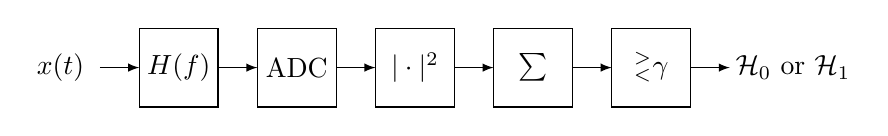
\begin{tikzpicture}
\node at (-5,3) {$x(t)$};
\node at (4.3,3) {$\mathcal{H}_0 \text{ or } \mathcal{H}_1$};
\draw [>=latex, ->] (-3,3) -- (-2.5,3);
\draw (-4,3.5) rectangle (-3,2.5) node[pos=.5]{$H(f)$};
\draw [>=latex, ->] (-4.5,3) -- (-4,3);
\draw (-2.5,3.5) rectangle (-1.5,2.5) node[pos=.5]{ADC};
\draw [>=latex, ->] (-1.5,3) -- (-1,3);
\draw (-1,3.5) rectangle (0,2.5) node[pos=.5]{$|\cdot|^2$};
\draw [>=latex, ->] (0,3) -- (0.5,3);
\draw (0.5,3.5) rectangle (1.5,2.5) node[pos=.5]{$\sum$};
\draw [>=latex, ->] (1.5,3) -- (2,3); 
\draw (2,3.5) rectangle (3,2.5) node[pos=.5]{$_<^ > \gamma$};
\draw [>=latex, ->] (3,3) -- (3.5,3);
\end{tikzpicture}
\caption{Conventional energy detector}\label{tkz:conv_ed}
\end{figure}
A standard digital energy detector is a detector that consists of a low-pass filter $H(f)$ that filters the analog input signal $x(t)$ such
that only the frequency band of interest remains\footnote{By using a mixer a lowpass filter can always be used to for this purpose}. This filtered signal is then converted to a digital signal $x[n]$ by an analog-to-digital converter (ADC). Then the detector takes the absolute value squared of each sample. The detector then estimates the energy $\Lambda$ of the signal during a period of $N$ samples by summing $N$ of those samples as
\begin{align}\label{eq:test_ed}
	\Lambda &= \sum_{n=0}^{N-1} |x[n]|^2.
\end{align}
This estimate is then compared to a threshold $\gamma$ to decide whether a signal other than noise is present in $x[n]$. That is, $\Lambda$ serves as test statistic for the binary hypothesis problem
\begin{align*}
	\begin{array}{ll}
		\mathcal{H}_0: & \text{if } \Lambda < \gamma, \\
		\mathcal{H}_1: & \text{if } \Lambda > \gamma.
	\end{array}
\end{align*}
The details behind determining the threshold $\gamma$ and a derivation of this energy detector can be found in \Cref{ssec:conv_ed_derivation}.

Some energy detectors use $\Lambda/N$ as test statistic\cite{chang2008sensing}, which is an estimate of the average power instead of the energy. Using this test statistic a detector that uses the autocorrelation $r_x[m]$ can be constructed. Such a detector is depicted in \cref{tkz:conv_ed}.
%  depends on the noise power $\sigma_n^2$  and the desired false alarm probability $p_{fa}$: the probability that the detector decides that hypothesis 2 is true, while hypothesis 1 is the true hypothesis. The derivation of $\gamma$ (see Appendix ...) gives the following result
% \begin{align*}
% \gamma = \left[Q^{-1}(p_{fa})\sqrt{N} + N\right]2\sigma_n^2
% \end{align*}
% where $Q^{-1}$ denotes the the inverse tail probability function of the standard normal distribution and $p_{fa}$ is the desired false alarm probability.
% As can be seen from  \cref{eq:test_ed} the test statistic used by the conventional energy detector does not take into account that the signal to be detected resides in a certain frequency band. Therefore it is necessary that the input signal $x[n]$ is filtered before $\Lambda$ is computed.
\begin{figure}[H]
\centering
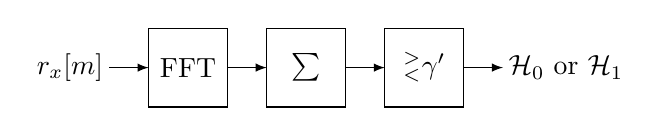
\begin{tikzpicture}
\node at (-2,3) {$r_x[m]$};
\node at (4.3,3) {$\mathcal{H}_0 \text{ or } \mathcal{H}_1$};
\draw [>=latex, ->] (-1.5,3) -- (-1,3);
\draw (-1,3.5) rectangle (0,2.5) node[pos=.5]{FFT};
\draw [>=latex, ->] (0,3) -- (0.5,3);
\draw (0.5,3.5) rectangle (1.5,2.5) node[pos=.5]{$\sum$};
\draw [>=latex, ->] (1.5,3) -- (2,3); 
\draw (2,3.5) rectangle (3,2.5) node[pos=.5]{$_<^ > \gamma'$};
\draw [>=latex, ->] (3,3) -- (3.5,3);
\end{tikzpicture}
\caption{Energy detector using the power spectral density}
\label{tkz:ed_psd}
\end{figure}
This detector calculates a discrete estimate of power spectral density by applying the Fast Fourier Transform to $r_x[m]$. By summating over the obtained power spectral density an estimate of the average power of $x[n]$ is obtained. This result is compared to a threshold $\gamma'$  to decide between $\mathcal{H}_0$ and $\mathcal{H}_1$. 

% As can be seen from \cref{eq:test_ed} the test statistic $\Lambda$ depends on the signal itself, not on the autocorrelation or the power spectral density which serves as input of our detector. We will now establish this relation by modifying the test statistic $\Lambda$.
% Let 
% \begin{align*}
% \Lambda' &= \frac{\Lambda}{N}\\
% 	&= \frac{\sum_{n=0}^{N-1} |x[n]|^2}{N},
% \end{align*}
% then $\Lambda'$ is an estimate of the average power $E\left[|x[n]|^2\right]$ of the signal $x$. We can use $\Lambda'$ as test statistic by using a modified threshold $\gamma' = \frac{\gamma}{N}$. To relate the power spectral density, which serves as input of our detector, to $\Lambda'$  we notice that by definition the integral over the power spectral density equals the expected average power:
% \begin{align}\label{eq:average_power_psd}
% E\left[\left|x[n]\right|^2\right] = \frac{1}{2\pi} \int_{-\pi}^{\pi}\mathcal{P}_x(\omega) \text{d}\omega.
% \end{align}
% Furthermore, by the Wiener-Khinchin theorem we have, if $x[n]$ is wide-sense stationary, that
% \begin{align}\label{eq:wiener_psd}
% 	\mathcal{P}_x(\omega) &= \mathcal{F}(r_x[n]) \\
% 	&= \sum_{n=-\infty}^{\infty} r_x[n] \exp [2\pi j\omega],
% \end{align}
% where the $\mathcal{F}(\cdot)$ denotes the Discrete Time Fourier Transform. 
% By combining \cref{eq:average_power_psd} and \cref{eq:wiener_psd} we can also relate the autocorrelation function to the test statistic $\Lambda'$. A energy detector using the test statistic is depicted in \cref{tkz:ed_psd}\footnote{it is assumed that $r_x[n]$ is based on an appropriate filtered signal}. A discrete power spectral density is estimated by applying the Fast Fourier Transform to $r_x[n]$. By summating over the obtained discrete power spectral density, an estimate of the average power is obtained. This estimate may then be compared with the threshold $\gamma'$.  
% \begin{figure}[H]
% \centering
% \begin{tikzpicture}
% \node at (-6.5,2.5) {$r_x[n]$};

% \draw [>=latex, ->] (-6,2.5) -- (-5.5,2.5);
% \draw (-5.5,3) rectangle (-4.5,2) node[pos=.5]{$\mathcal{F}$};

% \draw [>=latex, ->] (-4.5,2.5) -- (-3.5,2.5);
% \draw (-3.5,3) rectangle (-2.5,2) node[pos=.5]{$\int P_x$};

% \draw [>=latex, ->] (-2.5,2.5) -- (-2,2.5);
% \draw (-2,3) rectangle (-1,2) node[pos=.5]{$_<^ > \gamma$};

% \draw [>=latex, ->] (-1,2.5) -- (-0.5,2.5);
% \node at (0.3,2.5) {$\mathcal{H}_0 \text{ or } \mathcal{H}_1$};


% \draw [>=latex, ->] (-4,1) -- (-3.5,1);
% \draw (-3.5,1.5) rectangle (-2.5,0.5) node[pos=.5]{$\int P_x$};

% \draw [>=latex, ->] (-2.5,1) -- (-2,1);
% \draw (-2,1.5) rectangle (-1,0.5) node[pos=.5]{$_<^ > \gamma$};

% \draw [>=latex, ->] (-1,1) -- (-0.5,1);
% \node at (0.3,1) {$\mathcal{H}_0 \text{ or } \mathcal{H}_1$};


% \draw [>=latex, ->] (-4,-1) -- (-3.5,-1);
% \draw (-3.5,-0.5) rectangle (-2.5,-1.5) node[pos=.5]{$\int P_x$};

% \draw [>=latex, ->] (-2.5,-1) -- (-2,-1);
% \draw (-2,-0.5) rectangle (-1,-1.5) node[pos=.5]{$_<^ > \gamma$};

% \draw [>=latex, ->] (-1,-1)-- (-0.5,-1);
% \node at (0.3,-1) {$\mathcal{H}_0 \text{ or } \mathcal{H}_1$};

% \draw (-4,2.5) -- (-4,-1);


% \node at (-3,0.11) {\vdots};
% \node at (-1.5,0.11) {\vdots};
% \node at (0.3,0.11) {\vdots};

% \end{tikzpicture}
% \caption{Energy detection, multiple frequency bands}\label{tkz:my_ed}
% \end{figure}
% The implementations of the energy detector proposed up until now do not allow for detection in multiple frequency bands. We will now propose a such an energy detector, which is depicted in \cref{tkz:my_ed}. By integrating over a specific band $W$ in the PSD an estimate of the average power in that band is obtained. This estimate is then compared to a threshold $\gamma''$ to determine the presence of a signal in that band.

% Notice that if $x[n]$ contains only white noise, then its autocorrelation function equals a delta function: $r_x[n] = \sigma_n^2\delta[n]$, with $\sigma_n^2$ the noise power. Therefore the power spectral density of $x[n]$, denoted by $\mathcal{P}(\omega)$ equals  
%  \begin{align*}
%  \mathcal{P}_x(\omega) &= \mathcal{F}(r_x[n])\\
%   &= \sigma_n^2.
%  \end{align*} The power spectral density is constant. If we want to detect the presence of a signal in a certain frequency band $W$, we can make use of this characteristic. Let
%  \begin{align*}
%  \Lambda'' &= \int_W \mathcal{P}(\omega) \text{d}\omega
%  \end{align*}
% denote the test statistic to detect a signal in the frequency band $W$.
%  If we integrate the power spectral density of white noise over $W$ we obtain an average power of  $\frac{W}{2\pi} \sigma_n^2$. Therefore if we are to use $\Lambda''$ as test statistic, we have to use the modified threshold $\gamma'' = \frac{W}{2\pi} \gamma'$. 

%  If the power spectral density is estimated by a Fast Fourier Transform on $r_x[n]$, then an estimate of $\Lambda''$ can be obtained by summating
%  the estimate over the desired frequency band. This would in principle allow for per frequency detection. This detector, however, is flawed: note that by increasing the bandwidth one is summating over, one decreases the variance of the test statistic. Or the other way around: by decreasing the bandwidth to just one sample of the discrete power spectral density one increases the variance of the test statistic. Increasing the variance of the test statistic means that we cannot use $\gamma''$ to achieve our desired $p_{fa}$. 
 
% Furthermore, note that this detector also depends on the amount of samples $N$ that were used to calculate $\Lambda$. However, this poses a problem if the detector uses the estimated autocorrelation of the reconstructor: what is $N$?

% In signal processing the autocorrelation function $r_x[n]$ is usually estimated by 
% \begin{equation}\label{eq:acf_est}
% r_x[n] = \frac{1}{N-|n|}\sum_{m=\max(0,n)}^{N-1+\min(0,n)} x[m]\overline{x}[m-n]
% \end{equation}
% By \cref{eq:acf_est} we have that $r_x[0] = \sum_{n=0}^{N-1} |x[n]|^2 = \Lambda$. That is, $N$ should be the amount of samples needed to estimate $r_x[0]$ in case that \cref{eq:acf_est} is used. 
% The reconstructor does not use \cref{eq:acf_est}, instead it combines samples from multiple cosets, which obscures what the value of $N$ should be. 
% \todo{Derive threshold based on distribution of $r_x[0]$}

% \subsection{Noise variance}
% As indicated, knowledge of the noise variance is necessary for the energy detector to work. In practical situations this noise variance may be estimated from a reference measurement in an empty frequency band. 

\subsection{Energy detection with knowledge of the reconstructor}\label{ssec:ari_ed}
\begin{figure}[H]
\centering
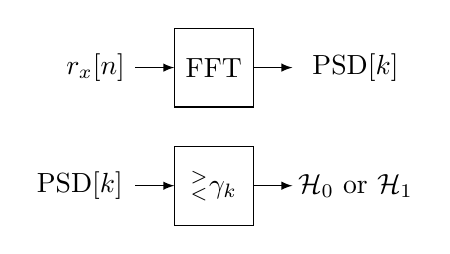
\begin{tikzpicture}

\node at (-3,4) {$r_x[n]$};

\draw [>=latex, ->] (-2.5,4) -- (-2,4);

\draw (-2,4.5) rectangle (-1,3.5) node[pos=.5]{FFT};

\draw [>=latex, ->] (-1,4) -- (-0.5,4);
\node at (0.3,4) {$\operatorname{PSD}[k]$};

\node at (-3.2,2.5) {$\operatorname{PSD}[k]$};

\draw [>=latex, ->] (-2.5,2.5) -- (-2,2.5);

\draw (-2,3) rectangle (-1,2) node[pos=.5]{$_<^ > \gamma_k$};

\draw [>=latex, ->] (-1,2.5) -- (-0.5,2.5);
\node at (0.3,2.5) {$\mathcal{H}_0 \text{ or } \mathcal{H}_1$};

\end{tikzpicture}
\caption{Energy detection with knowledge of the reconstructor}\label{tkz:ed_ari_overview}
\end{figure}
The problem with the conventional energy detectors as described above is that they assume that the signal is filtered to only contain the frequency band of interest. This filtering of  $x[n]$ however affects the reconstruction process of $r_x[m]$ and we can therefore not prefilter the signal. 

A modified energy detector as proposed in \cite{ariananda2012compressive} is depicted in \cref{tkz:ed_ari_overview}. The detector first estimates the power spectral density by applying the Fast Fourier Transform to an estimate of the autocorrelation function. This results in a discrete estimate of the power spectral density. Each element of this estimate is then compared an element-dependent threshold $\gamma_k$. As this detector detects per frequency whether there is a signal present or not, filtering of the signal is not necessary anymore.
To calculate $\gamma_k$ information about the reconstruction method as described in \Cref{cha:reconstruction} is used. Details on this calculation can be found in \cref{sec:ari_ed_deriv}.

% Let $\vec{s}_x \in \mathbb{R}^{2LN+1}$ denote the discrete power spectral density vector obtained by applying the $(2LN+1)$ point Discrete Fourier Transform to $\vec{r}_x$. 

% The vector $\vec{s}_x$ is then given by
% \begin{align}
% \vec{s}_x &= F_{(2NL+1)}\vec{r}_x
% \end{align}
% where $F_{(2NL+1)}$ denotes the $(2LN+1)\times (2LN+1)$ DFT matrix. 

% To determine the threshold $\gamma_{k}$ for each element of the $\vec{s}_x$, the signal $x[n]$ is assumed to contain only white noise. The distribution of the elements of the reconstructed power spectral density can then be approximated as a gaussian distribution \footnote{For the interested reader, see the Appendix \textbf{TODO} for a derivation}, which we will denote as $(\vec{s}_x)_k \sim \mathcal{N}(\mu_k, \sigma_k^2)$.
% Given $\mu_k$ and $\sigma^2_k$, the threshold for each frequency $\omega$ given a false alarm probability $p_{fa}$ can be calculated as by noting that:
% \begin{align}\label{eq:pfa_ari}
% p_{fa} &= P\left(E(s_k) > \gamma_k \big| \mathcal{H}_0\right) \\
% &= P\left(0 > \frac{\gamma_k -E(s_k)}{\Var(s_k)} \big| \mathcal{H}_0\right) \nonumber \\
% &= Q(\frac{\gamma_k -E(s_k)}{\Var(s_k)}) \nonumber.
% \end{align}
% The threshold $\gamma_k$ can then be obtained by solving \cref{eq:pfa_ari} for $\gamma_k$
% \begin{align*}
% \gamma_k &= Q^{-1}(p_{fa})\sigma_k + \mu_k.
% \end{align*}
% To obtain $\mu_k = E\left((\vec{s}_x)_k\right)$ notice that
% \begin{align}\label{eq:exp_sx}
% E\left(\vec{s}_x\right) &= \mat{F}\mat{R}^{\dagger}E\left(\vec{r}_y\right).
% \end{align} where the elements of $\vec{r}_y$ are given by 
% \begin{align}\label{eq:exp_ry}
% \vec{r}_{y_i, y_j}[k] &= (c_{i,j} \ast r_x)[mN]& \text{\cref{eq:cij-rx}} \\
% &= c_{i,j}[0]\delta[k]. \nonumber
% \end{align}
% Therefore $\mu_k$ can be obtained by evaluating the $k^{th}$ element of $E\left(\vec{s}_x\right)$ using \cref{eq:exp_sx} and \cref{eq:exp_ry}.
% Now that we have found $\mu_k$ we turn to the problem of finding $\sigma^2_k$. Let the covariance matrix of a vector $\vec{a}$ be defined as
% \begin{align}\label{eq:cov_mat}
% \mat{C}_a &= E(\vec{a}\vec{a}^H) - E(\vec{a})E(\vec{a}^H),
% \end{align}
% then element $C_{ij}$ is given by
% \begin{align}\label{eq:elem_cov_mat}
% C_{a_{ij}}&= \begin{cases}
% \Var(a_i, a_i) & \text{if } i=j\\
% \Cov (a_i, a_j) & \text{if } i\neq j.
% \end{cases}
% \end{align}
% Notice that the diagonal elements of a covariance matrix equal the variances of its corresponding vector. We will therefore compute the covariance matrix of $\vec{s}_x$ to obtain $\sigma_k^2$. Let the covariance matrix of $\vec{s}_x$ be denote by $\mat{C}_s$, then
% \begin{align*}
% \mat{C}_{s} &= E\left[\vec{s}_x\vec{s}_x^H\right] - E\left[\vec{s}\right]E\left[\vec{s}^H\right] \\
% &= E\left[\left(\mat{F} \mat{R}^{\dagger}\vec{r}_y\right) \left( \mat{F}\mat{R}^{\dagger}\vec{r}_y\right)^H\right] - E\left[\mat{F}\mat{R}^{\dagger}\vec{r}_y\right]E\left[\left(\mat{F}\mat{R}^{\dagger}\vec{r}_y\right)^H\right] \\
% &= \mat{F}\mat{R}^{\dagger} E\left[ \vec{r}_y\vec{r}_y^H\right]  \mat{R}^{\dagger H}\mat{F}^H -  \mat{F}\mat{R}^{\dagger} E\left[ \vec{r}_y\right] E\left[\vec{r}_y^H\right]   \mat{R}^{\dagger H}\mat{F}^H \\
% &= \mat{F}\mat{R}^{\dagger} \mat{C}_{r_y} \mat{R}^{\dagger H}\mat{F}^H
% \end{align*}
% where $\mat{C}_{r_y}$ denotes the covariance matrix of $\vec{r}_y$. The elements of $\mat{C}_{r_y}$ are given by\cite{ariananda2012compressive}
% \begin{align}\label{eq:elem_cov_ry}
% 	\Cov(r_{y_{rs}}[t], r_{y_{uv}}[w]) &= \frac{\sigma_n^4 c_{ru}[0]\conj{c}_{sv}[0]\delta[w-t]}{K-|t|}
% \end{align}

% \begin{figure}[H]
% \centering
% \begin{tikzpicture}

% \draw [fill=lightgray] (-2,0) rectangle (1,-1);
% \draw (1,3) rectangle (3,-1);
% \draw [fill=cyan, opacity=0.2] (1,3) rectangle (3,-1);
% \draw [fill=lightgray](3,0) rectangle (9,-1);


% \draw [>=latex,<->] (-2.1,-1) -- (-2.1,0);
% \node at (-2.4,-.5) {$\sigma^2_n$};

% \draw [red] (-2,.1) -- (9.2,.1);

% \draw [>=latex,<->] (9.2,-1) -- (9.2,.1);
% \node at (9.4,-.4 ) {$\gamma$};

% \node at (-2,-1.5) {0 rad/s};
% \node at (9,-1.5) {$2\pi$ rad/s};
% \end{tikzpicture}
% \caption{Energy detection with power spectral density}\label{tkz:ed_ari}
% \end{figure}

\section{Covariance absolute value method}

\begin{figure}[H]
\centering
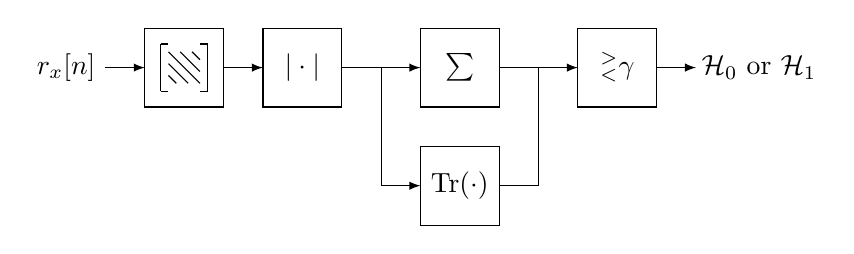
\begin{tikzpicture}

\node at (-4,4.5) {$r_x[n]$};

\draw [>=latex, ->] (-3.5,4.5) -- (-3,4.5);

\draw (-3,5) rectangle (-2,4) node[pos=.5]{};
\draw [>=latex, ->] (-2,4.5) -- (-1.5,4.5);

\draw (-1.5,5) rectangle (-0.5,4) node[pos=.5]{$|\cdot|$};
\draw [>=latex, ->] (-0.5,4.5) -- (0.5,4.5);

\draw (2.5,5) rectangle (3.5,4) node[pos=.5]{$_<^ > \gamma$};
\draw [>=latex, ->] (3.5,4.5) -- (4,4.5);

\draw (0.5,5) rectangle (1.5,4) node[pos=.5]{$\sum$};
\draw [>=latex, ->] (1.5,4.5) -- (2.5,4.5);

\draw (0.5,3.5) rectangle (1.5,2.5) node[pos=.5]{Tr($\cdot$)};

\node at (4.8,4.5) {$\mathcal{H}_0 \text{ or } \mathcal{H}_1$};

\draw (0,4.5) -- (0,3);
\draw (2,4.5) -- (2,3);
\draw (2,3) -- (1.5,3);
\draw [>=latex,->] (0,3) -- (0.5,3);

\draw (-2.6,4.3) -- (-2.7,4.4);

\draw (-2.45,4.3) -- (-2.7,4.55);
\draw (-2.3,4.3) -- (-2.7,4.7);
\draw (-2.3,4.45) -- (-2.55,4.7);

\draw (-2.3,4.6) -- (-2.4,4.7);

\draw (-2.8,4.8) -- (-2.8,4.2);
\draw (-2.8,4.8) -- (-2.7,4.8);
\draw (-2.8,4.2) -- (-2.7,4.2);

\draw (-2.2,4.8) -- (-2.2,4.2);
\draw (-2.2,4.2) -- (-2.3,4.2);
\draw (-2.2,4.8) -- (-2.3,4.8);


\end{tikzpicture}
\caption{CAV detector}\label{tkz:cav}
\end{figure}
The CAV detector was first introduced in \cite{zheng2009spectrum}. A block diagram of a CAV detector is depicted  in \cref{tkz:cav}, from which it can be seen that it performs 5 steps:
\begin{enumerate}[labelindent=0pt,labelwidth=\widthof{\ref{last-item3}},label=Step \arabic*:,itemindent=1em,leftmargin=!]
	\item Calculate the $L\times L$ symmetric toeplitz matrix $\mat{C}$ using the first $L$ samples of $r_x[n]$ as the first column. The matrix $\mat{C}$ is given by
	\begin{align}
		\mat{C} &= \begin{bmatrix}
		r_x[0] & r_x[1] & \ldots & r_x[L-1] \\
		r_x[1] & r_x[0] & \ldots & r_x[L-2] \\
		\vdots & \vdots & \ddots & \vdots \\
		r_x[L-1] & r_x[L-2] & \ldots & r_x[0]
		\end{bmatrix}.
	\end{align}
	\item Take the absolute value of all elements of $\mat{C}$.
	\item Calculate the sum of all elements, that is $T_1 = \sum_{n=1}^{L-1}\sum_{m=1}^{L-1} C_{nm}$.
	\item Calculate the trace of $\mat{C}$, that is $T_2 = \text{Tr}(\mat{C})$.
	\item Compare $T_1/T_2$ to a threshold $\gamma$. In case that $T_1/T_2 > \gamma$ it is decided that $\mathcal{H}_1$ is true, otherwise $\mathcal{H}_0$ is regarded as the true hypothesis.
    \label{last-item3}
\end{enumerate}

The threshold $\gamma$ is derived and an explanation of CAV can be found in \cref{sec:cav_derivation}.

\subsection{Filtering}
To be able to detect in a certain frequency band the input signal should be filtered by a band-pass filter. However if the input signal $x[n]$ is filtered, then the noise in that input signal is also filtered. This affects the autocorrelation function $r_x[n]$.  A technique to circumvent this problem is proposed in \cite{zheng2009spectrum}, but requires that the filter applied to $x[n]$ is known. However, we start our detection process with $r_x[n]$ instead of $x[n]$ and therefore cannot use this technique.  This limits the CAV implementation as described in this section to detection in just one frequency band. Furthermore, if use of this technique was possible, it would imply that we need to apply it per frequency band which may significantly add up to the computational cost in case that wide-band spectra are used.

% To determine the the threshold of the CAV detector we assume that the elements of the reconstructed auto correlation  $\hat{r}_x[n]$ are approximately gaussian distributed (see \cite{zheng2009spectrum} \cite{ariananda2012compressive}).

% However, unlike \cite{zheng2009spectrum} we cannot use the expression 
\end{document}